\documentclass[12pt,a4paper]{article}
\usepackage[utf8]{inputenc}
\usepackage[spanish]{babel}
\usepackage{amsmath}
\usepackage{amsfonts}
\usepackage{url}
\usepackage[sort, numbers]{natbib}
\usepackage[hidelinks]{hyperref}  % Hyperlinks bib references.
\usepackage{amssymb}
\usepackage{imakeidx}
\usepackage{graphicx}
\usepackage{tabularx}
\usepackage{footnote}
\usepackage{cancel}
\usepackage{xcolor}

\usepackage{listings}
\usepackage{listingsutf8}
\definecolor{mGreen}{rgb}{0,0.6,0}
\definecolor{mGray}{rgb}{0.5,0.5,0.5}
\definecolor{mPurple}{rgb}{0.58,0,0.82}
\definecolor{backgroundColour}{rgb}{0.95,0.95,0.92}

\lstdefinestyle{CStyle}{
    backgroundcolor=\color{backgroundColour},   
    commentstyle=\color{mGreen},
    keywordstyle=\color{magenta},
    numberstyle=\tiny\color{mGray},
    stringstyle=\color{mPurple},
    basicstyle=\footnotesize,
    breakatwhitespace=false,         
    breaklines=true,                 
    captionpos=b,                    
    keepspaces=true,                 
    numbers=left,                    
    numbersep=5pt,                  
    showspaces=false,                
    showstringspaces=false,
    showtabs=false,                  
    tabsize=2,
    language=C
}

%FOR DRAWING GRAPHS
\usepackage {tikz}
\usetikzlibrary {positioning}
\usepackage {xcolor}
\definecolor {processblue}{cmyk}{0.96,0,0,0}
\usetikzlibrary{arrows,topaths}

\usepackage{wrapfig}

%\usepackage[dvipsnames]{xcolor}
\newcommand\tab[1][1cm]{\hspace*{#1}}
\setlength{\parindent}{0pt}
\addto\captionsspanish{% Replace "english" with the language you use
  \renewcommand{\contentsname}%
    {Tabla de contenidos}%
}
\usepackage[left=2.54cm,right=2.54cm,top=2.54cm,bottom=2.54cm]{geometry}
\author{Antonio Morán Muñoz}
\title{Monitor de salud}
\usepackage{fancyhdr}
\pagestyle{fancy}
\lhead{MONITOR DE SALUD}
\rhead{\thepage}
\cfoot{Dispositivos y redes inalámbricos}
\renewcommand{\headrulewidth}{0.4pt}
\renewcommand{\footrulewidth}{0.4pt}
\begin{document} 

\begin{titlepage}
\thispagestyle{empty}
\centering
	
\includegraphics[width=0.35\textwidth]{castilla.png}\par\vspace{1cm}
	{\scshape\LARGE Universidad de Castilla-La Mancha \par}
	\vspace{1cm}
	{\scshape\Large Dispositivos y redes inalámbricos\par}
	\vspace{1.5cm}
	{\huge\bfseries SIGFOX: MONITOR DE SALUD\par}
	\vspace{2cm}
	{\Large\itshape Antonio Morán Muñoz\par}
	{\Large\itshape Pablo Olivas Auñón\par}

	\vfill

% Bottom of the page
	{CURSO ACADÉMICO 2018/2019}
	\vfill
	{\large \today\par}
\end{titlepage}

\thispagestyle{empty}
\newpage

\tableofcontents
\listoffigures

\newpage

\section{Objetivos del proyecto}
El objetivo del proyecto es poder monitorizar de forma sencilla y establecer un sistema de alertas para una serie de valores obtenidos de un paciente (por ejemplo número de pulsaciones por minutos, temperatura corporal, tensión o nivel de glucosa en sangre), no importando la ubicación del mismo.

\section{Diseño del proyecto}
La tecnología Sigfox nos permite enviar mensajes desde un emisor en casi cualquier parte del país hasta una desde la que podemos tratarlos y enviar alertas a multiples receptores. Esto es lo que nos ha permitido crear este monitor de salud basado en dicha tecnología.\\ 

Nuestro monitor de salud permite; tras obtener las pulsaciones, temperatura, tensión y nivel de glucosa en sangre; enviar estos dato con una cierta frecuencia a la nube de Sigfox, donde serán reenviados al centro de IOT de Azure para finalmente ser recibidos por nuestro servidor. Con los datos ya en manos del usuario final se distinguen dos usos diferenciados. Primero, tenemos una sistema de alertas para los receptores finales mediante un bot de Telegram, que recibirán si hay algún valor extraño en los datos obtenidos del paciente. El segundo uso consiste en una pequeña base de datos de fácil uso para poder visualizar el historial de todas las constantes del paciente.

\section{Desarrollo del proyecto}

\subsection{Arduino}

En el Listing \ref{a} podemos ver el código que se encargará de aleatorizar los valores para los diferentes parámetros que vayamos a monitorizar. El programa es muy sencillo. En la función de \textit{setup} configuramos el dispositivo establecemos la semilla para generar valores aleatorio. Tras esto, en la función \textit{loop}, lo que tenemos que hacer es declarar los diferentes parámetros a monitorizar e iniciarlos a un valor aleatorio. Tras esto, creamos un paquete en el que meteremos toda esa información y la enviaremos al backend de SigFox. La instrucción de la línea 47 suspenderá el dispositivo durante 10 segundos antes de volver a enviar un nuevo paquete.

\lstset{inputencoding=utf8/latin1}
\begin{minipage}{\linewidth} 
  \lstinputlisting[language=C,style=CStyle,caption={Codigo de Arduino},label={a}]{Arduino_Monitor.ino} 
\end{minipage}

\subsection{Configuración del callback}

El siguiente paso es configurar un nuevo callback en el backend de SigFox, que se encargue de enviar la información recibida del dispositivo y la redirija a Azure. Para ello, primero debemos crear una instancia de Azure IoT, con la configuración mostrado en la Figura \ref{acr}. En la Figura \ref{b} vemos la configuración del callback. En primer lugar, tenemos que indicar que es un uplink, ya que mandaremos la información a otro servicio. En segundo lugar, en el campo \textit{Custom payload config} indicamos cómo se deberán interpretar los datos encapsulados en el paquete que recibamos. En el campo \textit{Connection string} tenemos que indicar la cadena de conexión al IoT Hub de Azure donde se enviarán los datos, la cual ha sido obtenida de la instancia de Azure creada anteriormente tal y como se muestra en la Figura \ref{acl}. Por último, indicaremos el formato de salida de los datos en el campo \textit{JSON body}.


\begin{figure}[!h]
\begin{center}
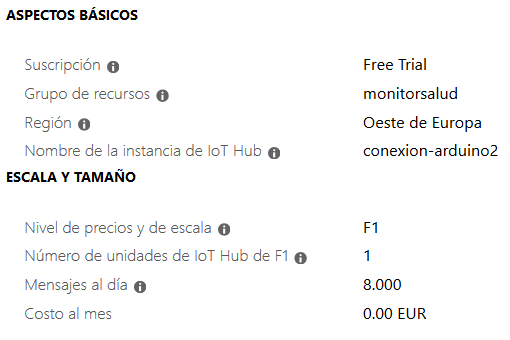
\includegraphics[width=300pt]{Azurecreacion.png}
\caption{Configuración del callback}
\label{acr}
\end{center}
\end{figure}

\begin{figure}[!h]
\begin{center}
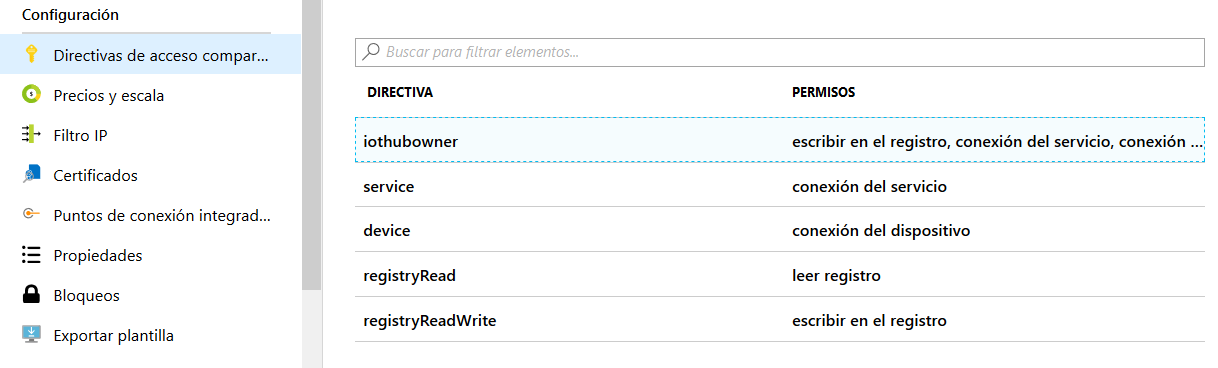
\includegraphics[width=\textwidth]{Azureclave.png}
\caption{Configuración del callback}
\label{acl}
\end{center}
\end{figure}

\begin{figure}[h!]
\begin{center}
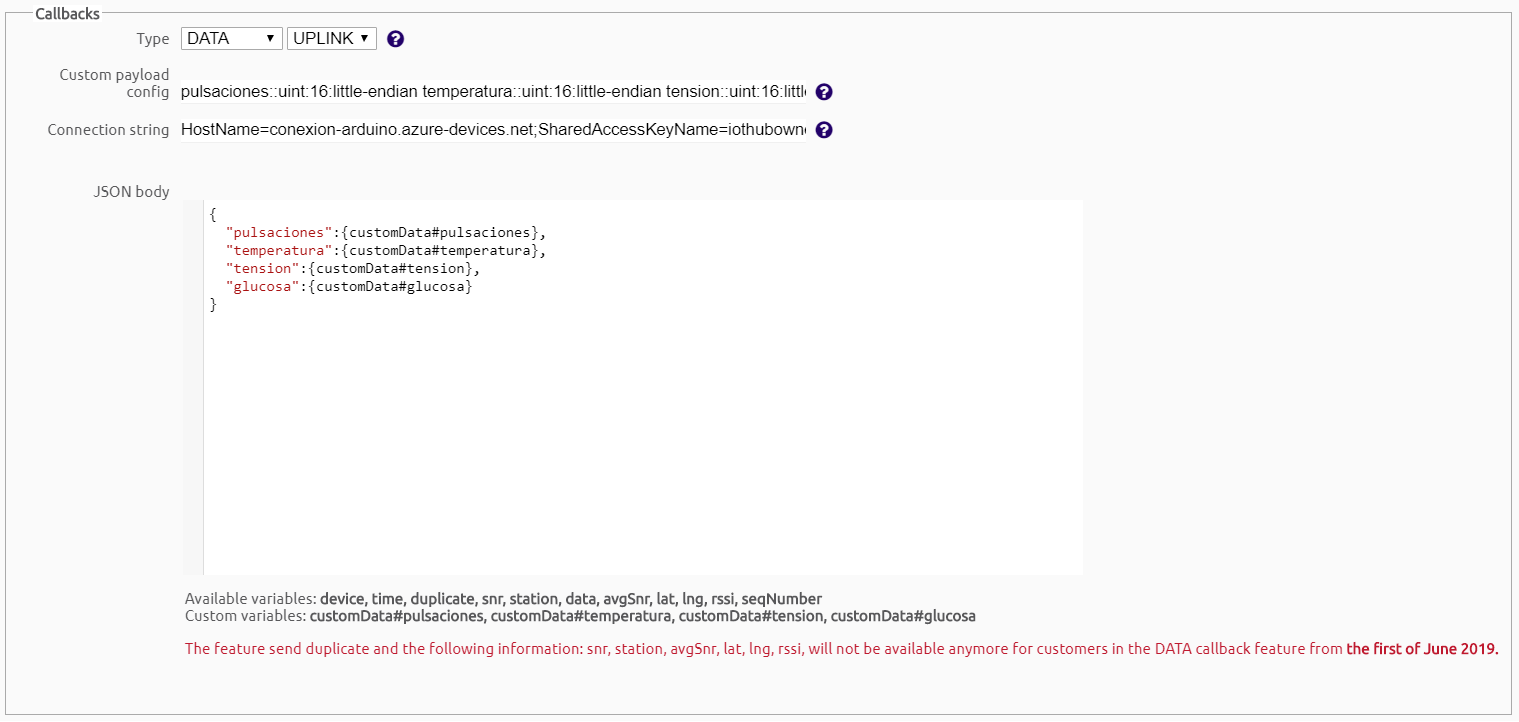
\includegraphics[width=\textwidth]{callback.png}
\caption{Configuración del callback}
\label{b}
\end{center}
\end{figure}

\subsection{Configuración del Bot}

A continuación, tenemos que crear el Bot que se encargará de la lógica del monitor. En el Listing \ref{c} se puede ver el código, que permite enviar la información recogida a una de Excel y mandar las notificaciones correspondientes a los valores anómalos.\\

\newpage
\lstset{inputencoding=utf8/latin1}
%\begin{minipage}{\linewidth}
  \lstinputlisting[language=C,style=CStyle,caption={Codigo del bot},label={c}]{bot.js}
%\end{minipage}


\section{Resultados y conclusiones}

Tras toda la configuración previa, podemos conectar el Arduino, meterle el código y ejecutarlo. El resultado de esto se puede ver en las siguientes figuras. En la Figura \ref{d} podemos observar cómo se han recibido las notificaciones por valores anómalos\\.\nocite{ref2}

\begin{figure}[!h]
\begin{center}
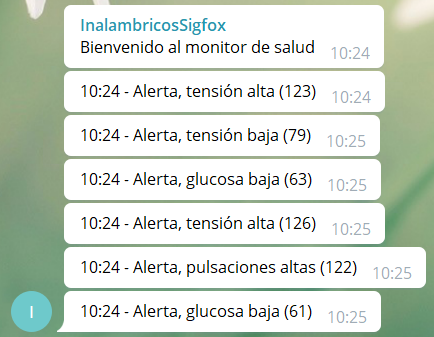
\includegraphics[scale=1]{notificaciones.png}
\caption{Notificaciones por Telegram}
\label{d}
\end{center}
\end{figure}


Una vez finalizado el proyecto, podemos establecer una serie de conclusiones acerca del uso de la tecnología SigFox. Esta tecnología es ideal para la esfera del IoT, como hemos visto por su capacidad de transmitir una pequeña cantidad de datos muy específicos que podrían representar cualquier característica del mundo real (en nuestro caso una serie de constantes vitales). Esta limitada capacidad de envío de datos permite un consumo mucho menor de energía, haciéndolo perfecto para aparatos que requieran de una gran autonomía. Por último, hay que destacar su área de cobertura que, si bien las hay mejores, es suficiente para abarcar numerosos casos de uso.

\newpage
\bibliographystyle{unsrtnat}
\bibliography{referencias}

\end{document}